\lhead{\emph{Background}}
\chapter{Background}
This chapter presents first different research areas and topics related to this thesis. Then in the second part related works are presented and compaired.


\section{Background overview}
From the problem statement of this thesis follows two main interaction goals: Hands-free interaction and eyes-free interaction. Common properties of these two areas are the topics and research areas related to this project. This overview is presented in fig. \ref{fig:venn}.

\begin{figure}[htbp]
	\centering
		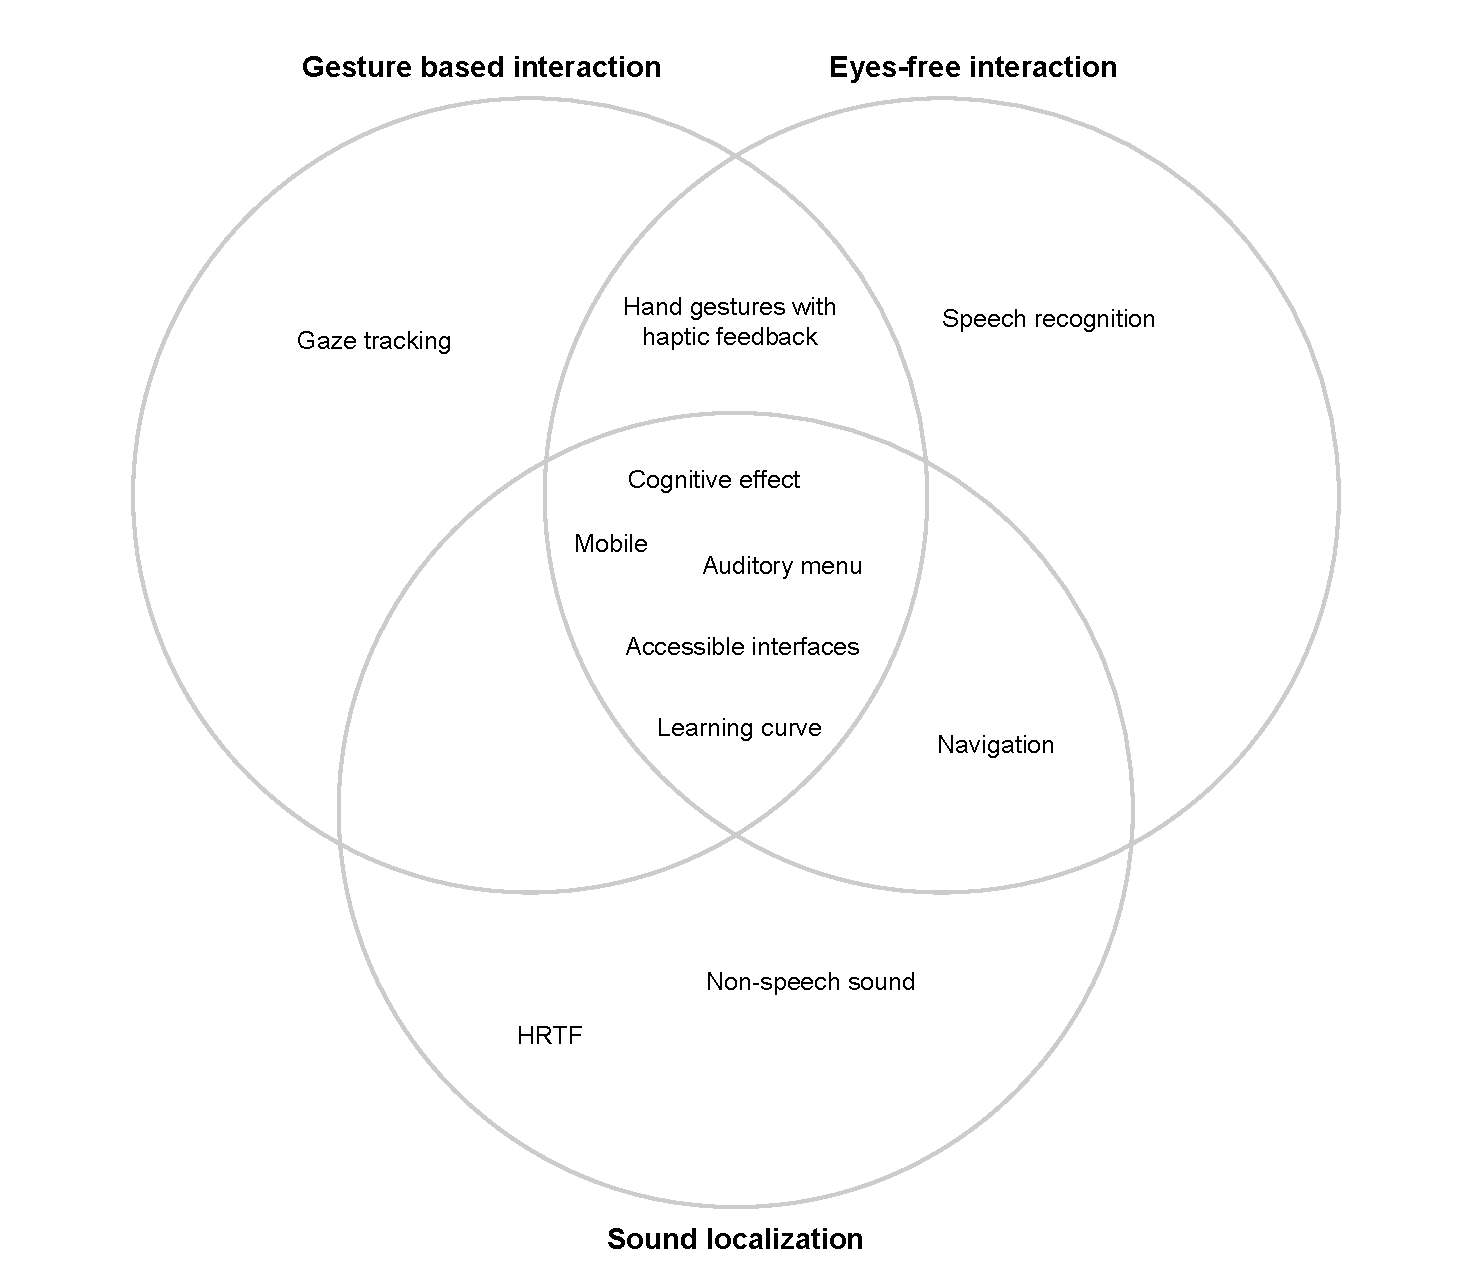
\includegraphics[width=\textwidth,height=\textheight,keepaspectratio]{./Figures/venn-diagram.pdf}
		\rule{35em}{0.5pt}
	\caption[Venn diagram]{A comparison of thesis topics}
	\label{fig:venn}
\end{figure}

\subsection{Hands-free interaction}
This term refers to controlling a system without using the hands including no hand gestures although sometimes used this way e.g. refers to not holding a device in the hand \cite{witt_designing_2006}. Achieving this hands-freeness interaction often relates to speech recognition or gaze/head tracking techniques but also other body parts are used for simple interactions e.g. leg shifting music track while running \cite{smus_running_2010}. Speech recognition is becoming a more common interaction modality but there exists accuracy and stability challenges especially in mobile noisy environments. In contrast head tracking could possibly provide a more stable interaction detection in mobile environments.

\subsection{Eyes-free interaction}
Several work on both audio \cite{kajastila_eyes-free_2013,bonner_no-look_2010,brewster_multimodaleyes-freeinteraction_2003,zhao_earpod:_2007,vazquez-alvarez_eyes-free_2011} and haptic \cite{pasquero_haptic_2011,pielot_tactile_2011} displays use the term eyes-free which refers to controlling the state of a system without visual attention. This kind of interaction has shown to be desirable in some situations \cite{oakley_designing_2007,yi_exploring_2012} and even improve efficiency compaired to traditional visual displays \cite{zhao_earpod:_2007}.

% visual competition, concentration
One of the main motivations behind this eyes-free use is to design interfaces that do not compete with the users visual attention. That is this "visual competition" could introduce risks when people are on the move e.g. travelling in traffic. In these situations a vital factor is to minimize the amount of distraction for interaction modes \cite{pascoe_using_2000}. Eyes-free interfaces can keep the users visual attention on the road while driving \cite{sodnik_user_2008} or walking around in the city \cite{vazquez-alvarez_eyes-free_2011}.

% visual display problems
Much of the interfaces work in wearable computing tends to focus on visual headmounted displays \cite{barfield_fundamentals_2000} e.g. Google Project Glass. But not only as mentioned does visual displays occupy the users visual attention, they can also be obtrusive and hard to use in bright daylight \cite{geelhoed_safety_2000}. Another disadvantage with visual displays is that their power consumption is high i.e. they drain a mobile device battery and they are expensive. By using eyes-free interfaces it is possible to use cheaper and less power consuming hardware.


\section{Spatial sound}
(Spatial audio, Head Related Transfer Function)...\\
Good reference for 3d sound \cite{begault_3dd_1994}

William W. Gaver, a pioneer in audio interfaces, has explored several aspects of using sound in interfaces including the intuitiveness of presenting complex information to users in the form of audio \cite{gaver_sonicfinder:_1989}. Similarly Graham explores the advantages in reaction time when using ”auditory icons” \cite{graham_use_1999}. In \cite{gaver_auditory_1986} Gaver presents the use of spatial sound icons. In doing so, he draws forward the unutilized potential of creating natural interaction through spatial audio.

Kajastila and Lokki has done a user study comparing auditory and visual menus controlled by the same free-hand gestures where the majority of the participants felt that an auditory circular menu was faster than a visual based menu \cite{kajastila_interaction_2013}.

Work has shown that non-speech audio is effective in improving the interaction with mobile devices \cite{pirhonen_gestural_2002, sawhney_nomadic_2000}.

By compairing visual and audio feedback when pushing buttons on the same GUI, Brewster showed that it was difficult for users to devote all their visual attention to an interface while walking, running og driving and that the interaction workload decreased with audio feedback \cite{brewster_overcoming_2002}.


\section{Head tracking}
There exists different kinds of areas when it comes to controlling a system with head gestures. Using cameras it is possible to effectively track head movements via facial recognition \cite{morimoto_recognition_1996} and gaze tracking makes it possible to control an object by fixating the eyes on that object while moving the head \cite{mardanbegi_eye-based_2012}. Thus these techniques do not require any hardware sensors e.g. accelerometer and gyroscope but in return a camera placed in front of the user. This will constrain the use especially in mobile "on-the-move" situations.

\subsection{Motion gesture recognition}
Dynamic Time Warping \cite{salvador_toward_2007}

\subsection{Intelligent Headset}
...


\section{Related work}
Based on the research areas and topics mentioned this section presents the specific related works in these areas and finally a sum up and comparison of the properties of the related works and this thesis.

% closely related to my project
Brewster et al. showed that novel interaction techniques based on sound and gesture can significantly improve the usability of a wearable device in particular under "eyes-free" mobile conditions and that head gestures was a successful interaction technique with egocentric sounds the most effective \cite{brewster_multimodaleyes-freeinteraction_2003}.

Park et al. also experimented, using head gesture input and aural output, with 1D and 2D menu interfaces \cite{park_gaze-directed_2011}.


\section{Sum up of related work and background}
Table: Summing up references that handles specific research areas...

\begin{table}[h] 
\caption{Related works properties comparison} % title name of the table 
%\centering % centering table

\begin{tabular}{L{3cm}C{2cm}C{2cm}C{2cm}C{2cm}} \toprule
    %{$m$} & {$\Re\{\underline{\mathfrak{X}}(m)\}$} & {$-\Im\{\underline{\mathfrak{X}}(m)\}$} & {$\mathfrak{X}(m)$} & {$\frac{\mathfrak{X}(m)}{23}$} & {$A_m$} & {$\varphi(m)\ /\ ^{\circ}$} & {$\varphi_m\ /\ ^{\circ}$} \\ \midrule
    Related work & Head gesture & Spatial sound & Music application & Accessible hardware \\ \midrule
    Multimodal eyes-free interaction techniques for wearable devices \cite{brewster_multimodaleyes-freeinteraction_2003}  & + & + & - & - \\ \bottomrule
    %2  & 3.442  & -2.509 & 3.442  & 0.299 & 0.343 & 133.2  & 152.4  \\
    %3  & 1.826  & -0.363 & 1.826  & 0.159 & 0.119 & 168.5  & -161.1 \\
    %4  & 0.993  & -0.429 & 0.993  & 0.086 & 0.08  & 25.6   & 90     \\ \midrule
    %5  & 1.29   & +0.099 & 1.29   & 0.112 & 0.097 & -175.6 & -114.7 \\
    %6  & 0.483  & -0.183 & 0.483  & 0.042 & 0.063 & 22.3   & 122.5  \\
    %7  & 0.766  & -0.475 & 0.766  & 0.067 & 0.039 & 141.6  & -122   \\
    %8  & 0.624  & +0.365 & 0.624  & 0.054 & 0.04  & -35.7  & 90     \\ \midrule
    %9  & 0.641  & -0.466 & 0.641  & 0.056 & 0.045 & 133.3  & -106.3 \\
    %10 & 0.45   & +0.421 & 0.45   & 0.039 & 0.034 & -69.4  & 110.9  \\
    %11 & 0.598  & -0.597 & 0.598  & 0.052 & 0.025 & 92.3   & -109.3 \\ \bottomrule
\end{tabular}

%\begin{tabular}{l c c c} % creating 10 columns 
%\hline\hline % inserting double-line 
%Related work & Head gesture & Spatial sound & Music application 
%\\ [0.5ex] 
%\hline % inserts single-line 
 
% Entering 1st row
%\cite{brewster_multimodaleyes-freeinteraction_2003} & X & X & [1ex]
%& &soft &1 & $-1$ & 1 & 1 & $-1$ & $-1$ & 1 \\[-1ex] 
%\raisebox{1.5ex}{Police} & \raisebox{1.5ex}{5}&hard 
%& 2 & $-4$ & 4 & 4 & $-2$ & $-4$ & 4 \\[1ex] 
 
% Entering 2nd row 
%& &soft & 1 & $-1$ & 1 & 1 & $-1$ & $-1$ & 1 \\[-1ex] 
%\raisebox{1.5ex}{Beethoven} & \raisebox{1.5ex}{5}& hard 
%&8 & $-8$ & 2 & 8 & $-8$ & $-8$ & 6 \\[1ex] 
 
% Entering 3rd row 
%& &soft & 1 & $-1$ & 1 & 1 & $-1$ & $-1$ & 1 \\[-1ex] 
%\raisebox{1.5ex}{Metallica} & \raisebox{1.5ex}{5}& hard 
%&4 & $-8$ & 8 & 4 & $-8$ & $-8$ & 8 \\[1ex] 
 
% [1ex] adds vertical space 
%\hline % inserts single-line 
%\end{tabular} 
\label{tab:related} 
\end{table}








